\documentclass[]{elsarticle}

\usepackage{amsmath}
\usepackage{xfrac}
\usepackage{xparse}
\usepackage{url}
\usepackage{hyperref}
\usepackage{subcaption}

\usepackage[inline,shortlabels]{enumitem}
\setlist[enumerate,1]{label=\textit{\alph*)}}


\DeclareDocumentCommand{\pddx}{mO{t}O{}}{\frac{\partial^{#3} {#1}}{\partial {#2}^{#3}}}
\newcommand{\w}{\omega}
\newcommand{\W}{\Omega}
\newcommand{\nbar}{\bar n}
\DeclareDocumentCommand{\ddt}{m}{\frac{\mathrm{d} {#1}}{\mathrm{d} t}}
\DeclareDocumentCommand{\bkt}{sm}{\IfBooleanTF{#1}{\left[ #2 \right]}{\left(#2\right)}}
\newcommand{\D}{\Delta}
\newcommand{\SD}[1]{\sigma\bkt*{#1}}
\DeclareDocumentCommand{\g}{s}{\gamma\IfBooleanT{#1}{_{eff}}}
\newcommand{\td}{\mathrm{d}}
\newcommand{\avg}[1]{\langle{#1}\rangle}
\newcommand{\wedm}{\w_{edm}}
\newcommand{\wimp}{\w_{\avg{E_v}}}
\newcommand{\wsw}{\w_{SW}}
\newcommand{\const}{\mathrm{const}}

\begin{document}
\title{Analysis of systematic errors in the frequency-based approach to estimating
  the deuteron electric dipole moment in a frozen spin storage ring}

\author[FZJ,INR,MEPHI]{Alexander Aksentev\corref{cor1}}
\ead{alexaksentyev@gmail.com}

\author[INR]{Yury Senichev}
\ead{y.senichev@inr.ru}

\author[MSU]{Eremey Valetov}
\ead{eremey@valetov.com}

\cortext[cor1]{Corresponding author}

\address[FZJ]{Institut f\"ur Kernphysik (IKP-2), Forschungszentrum J\"ulich,
 % 52428 Wilhelm-Johnen-Stra\ss{}e,
  J\"ulich, Germany}
\address[INR]{Institute for Nuclear Research of the Russian Academy of Sciences,
  %117312 60th October Anniversary pr. 7a,
  Moscow, Russia}
\address[MEPHI]{National Research Nuclear University ``MEPhI,''
  %115409 Kashira Highway 31,
  Moscow, Russia}
\address[MSU]{Department of Physics and Astronomy, Michigan State University,
  %220 Trowbridge Rd, East Lansing,
  MI 48824, USA}


\begin{abstract}
  The purpose of the present work is to evaluate the capability of the frequency-based approach
  to the measurement of the electric dipole moment of a charged particle in a storage ring environment.

  For that purpose, we analyzed several effects of the beam spin dynamics, which could result in systematic
  errors in the electric dipole moment estimator statistic. Those are: spin motion perturbations caused by
  betatron oscillations; spin decoherence in the frozen spin regime; properties of the magnetic dipole
  moment faking signal.
\end{abstract}


\maketitle

\textbf{Keywords:} electric dipole moment; frozen spin; spin transparency; spin dynamics; spin decoherence.


\section{Introduction}
One major question to be answered by current fundamental physics research is
the baryon asymmetry of the universe.
An answer to that question could be found in the violation of CP-symmetry, one
of the Sakharov conditions for baryogenesis. Permanent electric dipole moments (EDMs), if they exist,
violate both the P- and T-symmetries, and in consequence of the CPT-theorem, CP-symmetry.
The Standard Model (SM) predicts exceedingly small values for nucleon EDMs,
in the range of $10^{-33}$ to $10^{-31}~e\cdot$cm,
which is way below the current upper bound for the neuteron EDM,
with $d_n = 2.9\cdot 10^{-26}~e\cdot$cm. This implies that particle EDMs can serve as a powerful tool
for discovering physics beyond the SM. For example, CP-violations that are endemic in
supersymmetric teories (SUSY) are such as to span $d_n$ values in the range of
$10^{-29}$ to $10^{-24}~e\cdot$cm.~\cite{JEDI}

The idea of searching of a particle EDM in a storage ring (SR) environment appeared
during the development of the g-2 experiment~\cite{BNL:g-2:2001} in Brookhaven National Laboratory.

\subsection{The Frozen Spin concept}
TODO: introduce the invariant spin axis and spin tune concepts.\\

The dynamics of a spin-vector $\vec s$ in a magnetic field $\vec B$ and an electrostatic field $\vec E$
is described by the Thomas-BMT equation. Its generalized version, accounting for the effect of
the particle's electric dipole moment, can be written in the rest frame as:
\begin{subequations}
  \begin{align}
    \ddt{\vec s} &= \vec s\times \bkt{\vec\W_{MDM} +\vec\W_{EDM}}, \label{eq:TBMT_main}
    \intertext{where the magnetic (MDM) and electric (EDM) dipole moment angular velocities
      $\vec\W_{MDM}$ and $\vec\W_{EDM}$ }
    \vec\W_{MDM} &= \frac qm \bkt*{G\vec B - \bkt{G - \frac{1}{\gamma^2-1}}\frac{\vec E\times\vec\beta}{c}},\label{eq:TBMT_MDM} \\
    \vec\W_{EDM} &= \frac qm \frac\eta2 \bkt*{\frac{\vec E}c + \vec\beta\times \vec B}.\label{eq:TBMT_EDM}
  \end{align}
\end{subequations}
In the above equations, $m,~q,~G=(g-2)/2$ are, respectively, the mass, charge, and anomalous magnetic moment
of the particle; $\beta = \sfrac{v_0}{c}$ is its normalized speed; $\gamma$ its Lorentz-factor.
The EDM factor $\eta$ is defined by the equation $d = \eta\frac{q}{2mc}$, in which $d$ is the particle EDM,
$s$ its spin.

The Frozen Spin (FS) measurement concept consists in injecting a longitudinally-polarized beam
into a storage ring having a radial electric field component
$E_r = \frac{GB_yc\beta\gamma^2}{1-G\beta^2\gamma^2}$,~\cite[p.~10]{BNL:Deuteron2008} so that the
magnetic dipole moment (MDM) component in~\eqref{eq:TBMT_main} is set to zero: $\vec\W_{MDM} = \vec 0$.
Then, any tilting of the beam polarization vector out of the horizontal plane
is attributed to the presence of an EDM. Specifically, the vertical polarization component
\begin{equation}\label{eq:Py_growth}
 P_y = A\cdot \sin\bkt{\underbrace{\sqrt{(\wedm + \wimp)^2 + \w_y^2 + \w_z^2}}_{\W}\cdot t + \delta}.
\end{equation}
In the above equation, $\wimp$ denotes the MDM spin precession frequency generated by fields connected
with machine imperfections.

\section{The frequency-based approach}
TODO: introduce the concept of spin wheel.\\

A brief summary of the approaches to the EDM measurement problem, within the FS paradigm.

According to equation~\eqref{eq:Py_growth}, we can conceptualize two distinct measurement modes:
\begin{enumerate*}
\item the amplitude-, and
\item the frequency-based methods.
\end{enumerate*}

In the former, all EDM-unrelated precession in the ring must first be suppressed; then, if the beam's
polarization vector still keeps turning, it indicates to us that something else (the EDM) exists,
that's turning it.

In the frequency-based methodology, spin precession is stopped only in the beam orbit plane, and the EDM
indicator is the change to the vertical plane spin precession frequency under time reversal (which is
performed via reversing the beam circulation direction).

Three advatages follow from not freezing the spin precession in the vertical plane:
\begin{enumerate}[(i)]
\item since we don't have to stop vertical plane MDM spin precession, lattice optical element alignment
  specifications aren't as stringent;
\item it also means that the spin precession axis is more stable, which is a remedy for another major
  systematic error -- geometric phase;\label{itm:advantages:stability}
\item and since we don't have to measure microradian deviations of the polarization vector from the
  beam orbit plane, the polarization measurement is much easier.
\end{enumerate}

\section{Betatron oscillations}

\subsection{Probem statement}
The problem of the betatron motion is as follows:
\begin{enumerate}
\item the EDM statistic is composed from two estimates of the spin precession frequency;
  in one the EDM and MDM effects add up, in the other subtract:
  \begin{equation*}
    \begin{cases}
      \hat\w_{edm} &= \frac12(\hat\w_x^+ + \hat\w_x^-),\\
      \w_x^\pm &= \w_{edm} \pm \w_{mdm}.
    \end{cases}
  \end{equation*}
\item Those frequencies are estimated via fitting a harmonic function with constant parameters to
  polarimety data:
  \begin{equation*}
    \begin{cases}
      f(t) &= a\cdot\sin(\w_x\cdot t + \delta)\mapsto \hat\w_x,\\
      (a,\w_x,\delta) &= \const.
    \end{cases}
  \end{equation*}
\item At the same time, the solution of the T-BMT equation for the vertical spin vector component
  has a non-constant amplitude $a = \sqrt{\nbar_x^2 + (\nbar_y\cdot\nbar_z)^2}$
  for a betatron-oscillating particle.
\end{enumerate}

\subsection{Simulation setup}
In the simulation we used a FS lattice with bent E+B-field spin rotators
shown in Figure~\ref{fig:BNL_lattice}.
We used an imperfect machine; imperfections were simulated by spin-rotator tilts about the optic axis.
The tilt angles were normally-diftributed, each trial the expectation of the tilt distribution was varied.
The non-zero expectation value simulates the application of a spin wheel driver.
Imperfections introduced in this way affect only the particle spin dynamics,
leaving the orbital dynamics the same for every trial.

\begin{figure}[h]
  \includegraphics[width=\linewidth]{img/BNL_lattice}
  \caption{Frozen Spin lattice used in all simulations. Bent E+B-field spin-rotators are inserted
    into the arc sections. The lattice length is 146 m,
    the beam injection energy is 270 MeV. Image taken from~\cite{Senichev:Lattices}.\label{fig:BNL_lattice}}
\end{figure}


Particles injected into the alttice were betatron-scillating in the vertical plane for the most part.
Since 270 MeV is not exactly the FS energy\footnote{The more precise value is 270.0092 MeV}
for this lattice, the radial component of the spin precession axis is fairly small. This, however,
does not pose a problem for this particular simulations, since it only amplifies the effect of vertical
betatron oscillations, which were being studied.

In the analysis we used three data sets. The $s_y^{trk}$ time series was taked directly
from the COSY Infinity~\cite{COSYInf} tracker. The $s_y^{gen}$ were data generated using a harmonic function
with varying amplitude and frequency; the amplitude and frequency values at time $t$ were computed based
on the invariant spin axis and spin tune time series obtained during COSY Infinity tracking.
The $s_y^{idl}$ data seres was also computed from the harmonic signal, but constant estimates of
amplitude and frequency were used.

From the data series, two comparator statistics/residuals were computed:
\begin{align*}
  \epsilon_1(t) &= s_y^{gen}(t) - s_y^{idl}(t), \tag{generator residual}\\
  \epsilon_2(t) &= s_y^{trk}(t) - s_y^{idl}(t). \tag{tracker residual}
\end{align*}

The tracker residual serves as an estimate of the amplitude oscillations
caused by the particle's betatron motion, and hence it is the primary statistic for analysis.

\subsection{Simulation results and conclusions}

In Figure~\ref{fig:smp:resid_vs_time} are shown the time-dependencies of the comparator
residuals. These are plots for the particle with the largest (3 mm) amplitude of betatron oscillations.
We observe that even in this case the tracker residual's oscillation amplitude does not exceed
$10^{-5}$; for a whole ensemble of particles, this value can only be smaller, due to the averaging effect.

The amplitude growth in the generator residual's case is due to the difference between the ideal
and generator signal's oscillation frequencies, which is a consequence of the way in which we defined the
ideal signal's parameters.
\begin{figure}[h]
  \includegraphics[width=\linewidth]{img/smp_sim/residual_vs_time(both)}
  \caption{Comparator statistics' time-dependence.\label{fig:smp:resid_vs_time}}
\end{figure}

Figure~\ref{fig:smp} presents the most significant simulation results. We make two observations:
\begin{enumerate}[(1)]
\item the comparator's standard deviations follow the same functional dependence on the SW driver's
  strength as the spin tune's, and do not show any interest in the behavior of the spin precession axis;
\item the variability of the precession axis grows smaller as the driver strength increases. This is
  what we referred to as advantage~\ref{itm:advantages:stability} of the frequency-based approach.
\end{enumerate}

\begin{figure}[h]\centering
  \begin{subfigure}{\linewidth}
    \includegraphics[width=\linewidth]{img/smp_sim/residual_SD_vs_SW(both)}
    \caption{Standard deviations of the comparator statistics versus the SW driver's
    relative strength.\label{fig:smp:resid}}
  \end{subfigure} 
  \begin{subfigure}{\linewidth}
    \includegraphics[width=\linewidth]{img/smp_sim/NBAR_variation_sd_vs_SW}
    \caption{The same statistic for the spin precession axis components and spin tune.\label{fig:smp:NBAR}}
  \end{subfigure}
  \caption{Effect of betatron oscillations on the particle spin dynamics simulation results.\label{fig:smp}}
\end{figure}

This simulation was set up so as to check the robustness of the frequency-based approach's EDM statistic
with regard to perturbations to the particle spin dynamics; specifically, those that cause the invariant
spin axis to change its orientation. Even though the only source of perturbation we used was
the particles' betatron motion, some general conclusions can be inferred from the results:
\begin{enumerate}[(1)]
\item The amplitude oscillations are small, as evidenced by Figure~\ref{fig:smp:resid_vs_time} (directly),
  and the residual standard deviation plots in Figure~\ref{fig:smp:resid} (indirectly). We expect the
  random polarization measurement error to occur at the percent level, which means that the superposition
  of this systematic error with the random measurement error should not exhibit any
  statistically-significant systematicity.
\item The correllation coefficient between the $\hat a$- and $\hat\w_x$-estimates is less than 10\%.
  The measured signal's amplitude oscillations affect the amplitude estimate in the first place, while
  their effect on the frequency estimate is described by the correllation coefficient. Since it is small,
  even if our first conclusion is false, and the amplitude oscillations are sufficient to bias the
  $\hat a$-estimate, their effect on the frequency estimate will be attenuated by at least a factor of 10.
\item This systematic effect is controllable. This can be observed in Figure~\ref{fig:smp:NBAR}, where
  the precession axis' variability goes down with the SW roll rate. The frequency-based approach permits
  the application of a SW driver in a reasonably wide strength range.
\end{enumerate}

\section{Spin decoherence}
\subsection{Origins}
According to equation $\nu_s = \gamma G$, a particle's spin tune depends on its energy. Because particles in
a bunch travel different length orbits, their equilibrium energy levels also experience a dispersion. As a
consequence, their spin vectors precess at different rates, which is the immediate cause of decoherence.

In Figure~\ref{fig:long_phase_port_3} one can see the longitudinal phase space portraits of particles
doing betatron oscillations in the verticel plane. The centers of the ellipses indicate the particles'
equilibrium energy levels. Data used in the drawing of this figure was obtained in a simulation in which
third-order spin and orbital transfer maps were utilized. Compare with the linear theory prediction, represented
in Figure~\ref{fig:long_phase_port_1}.

\begin{figure}[h]\centering
  \begin{subfigure}{\linewidth}
    \includegraphics[width=\linewidth]{img/decoh/psp_diagram_betatron}
    \caption{Particles do vertical plane betatron oscillations.
      Colors mark the particles' vertical offsets at injection; all other initial coordinate offsets are zero.
      Third-order transfer maps were used in the computation of this plot's data.\label{fig:long_phase_port_3}}
  \end{subfigure}
  \begin{subfigure}{\linewidth}
    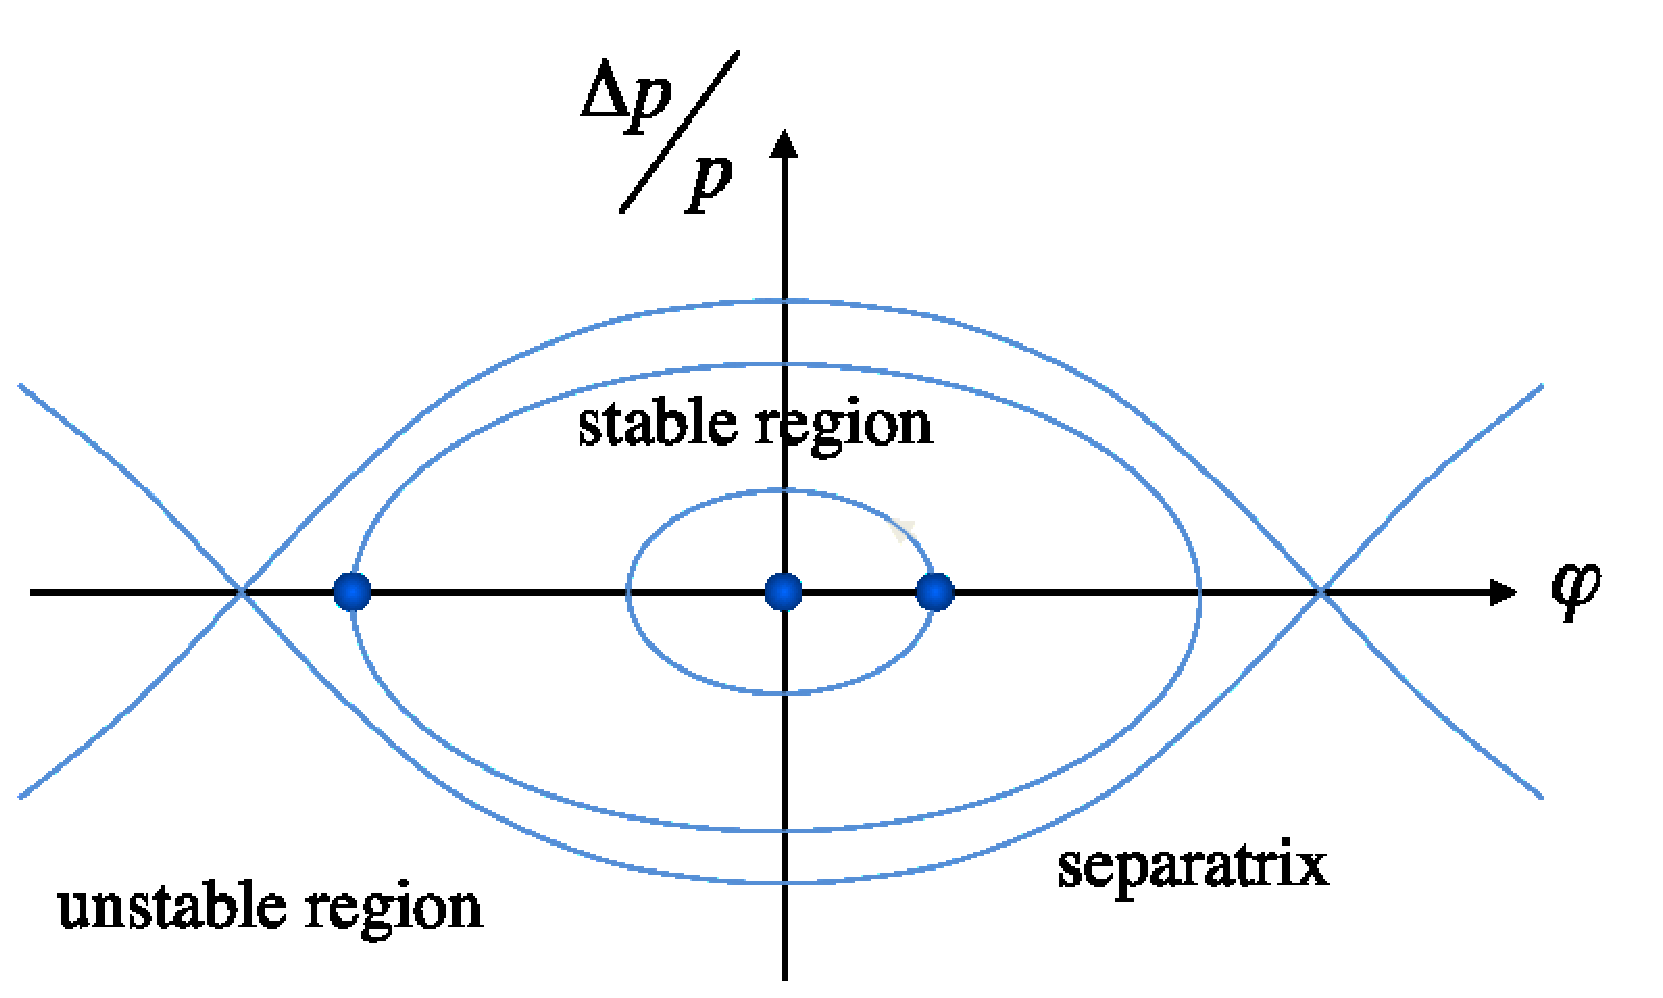
\includegraphics[width=\linewidth]{img/decoh/psp_diagram.eps}
    \caption{Classic text-book image computed from a linear theory. All ellipses are centered
    on one point, i.e. all particles have the same equilibrium energy.\label{fig:long_phase_port_1}}
  \end{subfigure}
  \caption{Longitudinal phase space portraits in a lattice using RF bunching.}
\end{figure}

\subsection{Theory behind the sextupole decoherence suppression technique}
Our hypothesis is that decoherence is a result of the dispersion in the particle equilibrium energy levels.
If one solves the system of equations for the longitudinal particle dynamics,~\footnote{For details,
  please cf. reference~\cite{Aksentev:IPAC19:Decoh}.} assuming a non-linear mometnum compaction factor
$\alpha = \alpha_0 + \alpha_1\cdot\delta$, one will obtain the following general expression
for the equilibrium level momentum shift:
\begin{equation}\label{eq:equ_mom_shift}
  \Delta\delta_{eq} = \frac{\gamma_0^2}{\gamma_0^2\alpha_0 - 1}\bkt*{\frac{\delta_m^2}{2}\bkt{\alpha_1 - \alpha_0\gamma^{-2}_0 + \gamma_0^{-4}} + \bkt{\frac{\Delta L}{L}}_\beta}.
\end{equation}

In the above equation:
\begin{enumerate}
\item $\delta = \D p/p$ is the particle's momentum offset~\footnote{$\delta_m$ is
  the amplitude of synchrotron oscillations.};
\item $\gamma_0$ is the Lorentz factor of the reference particle;
\item $\bkt{\frac{\D L}{L}}_\beta = \frac{\pi}{2L}\bkt*{\epsilon_xQ_z + \epsilon_yQ_y}$ is the
  orbit lengthening due to betatron oscillations;
\item $\epsilon_{x,y}$ are, respectively, the horizontal and vertical transverse emittances, $Q_{x,y}$ the
  corresponding betatron tunes.
\end{enumerate}

The expression~\eqref{eq:equ_mom_shift} contains two terms: the first has to do with
the non-linear momentum compaction factor, the second with the particle orbit length.

If one inserts a sextupole of strength
\begin{align}
  S_{sext} &= \frac{1}{B\rho} \pddx{B_y}[x][2]
  \intertext{into the beam line, its field will first of all affect the particle trajectories:}
  \bkt{\frac{\Delta L}{L}}_{sext} &= \mp \frac{S_{sext}D_0\beta_{x,y}\varepsilon_{x,y}}{L} \label{eq:sext:OL_effect},
  \intertext{and second --- it will modify the non-linear part of the momentum compaction factor:}
  \Delta \alpha_{1,sext} &= -\frac{S_{sext}D_0^3}{L}. \label{eq:sext:MCM_effect}
\end{align}
We call equation~\eqref{eq:sext:OL_effect} the {orbit length effect},
equation~\eqref{eq:sext:MCM_effect} the {momentum compaction factor effect}.
In the following sections we will try to analyze the signatures of these effects in spin tune data.

\subsection{Sextupole field effect signatures}
\subsubsection{Momentum compaction factor effect}

In Figure~\ref{fig:sext:MCM_effect} is drawn the dependence of a particle's mean spin tune level
on its mean energy level. In this simulation we injected an ensemble of particles with differing
initial energy offsets on the closed orbit of the FS lattice from Figure~\ref{fig:BNL_lattice}.
Since the sextupole fields do not affect the closed orbit, this simulation tests only for the
momentum compaction factor effect. 

The plot exhibits two features:
\begin{enumerate}[(1)]
\item the functional dependence $\avg{\nu_s}(\avg{\D K/K})$ changes with the field gradient;
  \item the point density distribution does not vary.
\end{enumerate}

In Figure~\ref{fig:sext:MCM_effect:LPS} we drew the particles' longitudinal phase space portraits.
We observe no change in the portraits when the sextupole field gradient is varied,
which is attributed to the particle orbit lengths' not changing.

\begin{figure}[h]\centering
  \begin{subfigure}{\linewidth}
    \includegraphics[width=\linewidth]{img/decoh/STDK_3SS_D}
    \caption{Dependence of the mean level of a particle's spin tune on its mean energy level.
      Colors mark different sextupole field gradients.
      The functional form of the dependence changes with the field strength.\label{fig:sext:MCM_effect}}
  \end{subfigure}
  \begin{subfigure}{\linewidth}
    \includegraphics[width=\linewidth]{img/decoh/LPS_3SS_D}
    \caption{Longitudinal phase space portraits of the injected particles.
      Particles were injected on the closed orbit, hence the sextupole fields do not affect their orbit length.
      No change is observed when the field strength changes.\label{fig:sext:MCM_effect:LPS}}
  \end{subfigure}
  \caption{Analysis of the sextupole fields' momentum compaction factor effect.}
\end{figure}

\subsubsection{Orbit length effect}
In this simulation, particles were injected at the same initial energy, but different vertical offsets
from the closed orbit. Because of that, they do betatron oscillations, and as a result, synchrotron oscillations.
As a consequence of equation~\eqref{eq:equ_mom_shift}, we should anticipate both sextupole field effects
in this simulation.

As predicted, Figure~\ref{fig:sext:OL_effect} exhibits two features:
\begin{enumerate}[(1)]
\item the functional dependence $\avg{\nu_s}(\avg{\D K/K})$ changes as in the previous simulation;
\item the point density distribution changes also.
\end{enumerate}

In Figure~\ref{fig:sext:OL_effect:LPS} we see that the phase portraits compress when the sextupole field gradient
is changed. This compression corresponds to the point density change, seen in Figure~\ref{fig:sext:OL_effect}.
\begin{figure}[h]\centering
  \begin{subfigure}{\linewidth}
    \includegraphics[width=\linewidth]{img/decoh/STDK_3SS_Y}
    \caption{Dependence of the mean level of a particle's spin tune on its mean energy level.
      Colors mark different sextupole field gradients.
      The functional form of the dependence changes with the field strength.\label{fig:sext:OL_effect}}
  \end{subfigure}
  \begin{subfigure}{\linewidth}
    \includegraphics[width=\linewidth]{img/decoh/LPS_3SS_Y}
    \caption{Longitudinal phase space portraits of the injected particles.
      Particles were injected on different betatron orbits, hence sextupole fields modify their orbit lengths.
      Portraits compress when the fields strength is varied.\label{fig:sext:OL_effect:LPS}}
  \end{subfigure}
  \caption{Analysis of the sextupole fields' orbit length effect.}
\end{figure}

\subsubsection{Conclusions}
The above analysis brought us to the following conclusions:
\begin{enumerate}[(1)]
\item The signature of the sextupole fields' momentum compaction factor effect is the change in the functional
  form of the mean spin tune dependence on the particle's mean energy level $\avg{\nu_s}(\avg{\D K/K})$.
  \item The pure orbit length effect is the reduction in the dispersion of the mean energy levels.
\end{enumerate}

Contrary to our original intuition, the minimization of the dispersion in the mean energy levels does not
effect the desired minimization in the dispersion of the perticles' spin tunes.
In Figure~\ref{fig:sext:OL_effect}, for example, we see that the sextupole gradient value corresponding to the
minimal $\SD{\D K/K}$ is not optimal in terms of $\SD{\avg{\nu_s}}$, while ar the optimal value,
the $\D K/K$ dispersion does not matter at all.


\section{MDM faking signal}


\begin{thebibliography}{9}

\bibitem{JEDI}
  JEDI Collaboration. \url{http://collaborations.fz-juelich.de/ikp/jedi/about/introduction.shtml}

\bibitem{BNL:g-2:2001}
  Brown HN, Bunce G, Carey RM, Cushman P, Danby GT, Debevec PT, et al.
  Precise measurement of the positive muon anomalous magnetic moment. PhysRevLett. 2001;86:2227–31. 

  
\bibitem{BNL:Deuteron2008}
  D. Anastassopoulos et al., ``AGS Proposal: Search for a permanent electric dipole moment of
  the deuteron nucleus at the $10^{-29}$ e$\cdot$cm level,'' BNL, 2008.

\bibitem{COSYInf}
  M. Berz, K. Makino, COSY INFINITY 10.0 Beam Physics Manual.

\bibitem{Mane:SpinWheel}
  S. Mane, ``A distillation of Koop's idea of the Spin Wheel,'' arXiv:1509.01167 [physics]
  \url{http://arxiv.org/abs/1509.01167}.

\bibitem{BNL:Proton}
  V. Anastassopoulos et al., ``A Storage Ring Experiment to Detect a Proton Electric Dipole Moment.''
  Rev. Sci. Instrum., 87(11), 2016.
  \url{http://arxiv.org/abs/1502.04317}.

\bibitem{Koop:SW}
  I. Koop. ``Asymmetric energy colliding ion beams in the EDM storage ring,'' Proc. of IPAC13 (2013).
  \url{http://accelconf.web.cern.ch/accelconf/ipac2013/papers/tupwo040.pdf}.

\bibitem{Aksentev:Stats}
  A. Aksentev, Y. Senichev. ``Statistical precision in charged particle EDM search in storage rings.''
  2017 J. Phys.: Conf. Ser. 941 012083.

\bibitem{Aksentev:IPAC19:SMP}
  A. Aksentev, Y. Senichev, ``Spin Motion Perturbation Effect on the EDM Statistic
  in the Frequency Domain Method,'' presented at the 10th International Particle Accelerator Conf. (IPAC'19),
  Melbourne, Australia, May. 2019, paper MOPTS011.

\bibitem{Senichev:FDM}
  Y. Senichev, A. Aksentev, A. Ivanov, E. Valetov, ``Frequency domain method of the search for
  the deuteron electric dipole moment in a storage ring with imperfections,'' arxiv:1711.06512 [physics.acc-ph]
  \url{https://arxiv.org/abs/1711.06512}.

\bibitem{Senichev:Lattices}
  Y. Senichev, S. Andrianov, S. Chekmenev, M. Berz, E.Valetov. ``Investigation of Lattice for Deuteron EDM Ring,''
  Proc. of ICAP15 (2015). \url{http://accelconf.web.cern.ch/AccelConf/ICAP2015/papers/modbc4.pdf}.

\bibitem{Eremey:Thesis}
  E. Valetov, ``Field modeling, symplectic tracking, and spin decoherence for the EDM and muon g-2 lattices.''
  PhD tehsis, Michigan State University, Michigan, USA.
  \url{http://collaborations.fz-juelich.de/ikp/jedi/public_files/theses/valetovphd.pdf}.

\bibitem{Aksentev:IPAC19:Decoh}
  A. Aksentev, Y. Senichev, ``Spin decoherence in the Frequency Domain Method for the search of a particle EDM,''
  presented at the 10th International Particle Accelerator Conf. (IPAC'19), Melbourne, Australia,
  May. 2019, paper MOPTS012.

\bibitem{Senichev:IPAC13}
  Y. Senichev et al., ``Spin tune decoherence effects in Electro- and Magnetostatic Structures.''
  Proceedings of IPAC 2013, Shanghai, China, pp. 2579-2581.

\bibitem{Aksentev:IPAC19:GFF}
  A. Aksentev, Y. Senichev, ``Simulation of the Guide Field Flipping Procedure for the Frequency Domain Method,'' 
  presented at the 10th International Particle Accelerator Conf. (IPAC'19), Melbourne, Australia,
  May 2019, paper MOPTS010.

\bibitem{Pretz:Stats:Sparse}
  J. Pretz, ``Determination of polarization and frequency parameters on sparse data,'' JEDI internal
  note \#2013/04, Sept. 23, 2013.
  
\bibitem{Aksentev:FDM}
  A. Aksentev, Y. Senichev, E. Valetov, JEDI internal note \#4/2019.
  
\end{thebibliography}

\end{document}
